\begin{flushleft}
    Die Software, die auf dem ESP32 ausgeführt besteht aus 3 Teilen. Zuerst werden die verschiedenen Pins initialisiert, anschließend werden die ROS Komponenten initialisiert. Danach wartet der Roboter auf eingehende Messages und führt die Befehle entsprechend aus.
    Beim Initialisieren der Pins wird zuerst der richtige Modus gesetzt. Anschließend wird ein Timer konfiguriert, der für die PWM-Signale an die Motoren verwendet wird.
    Zum Ende der ersten Phase werden die PWM Channels mit den entsprechenden Pins und dem Timer eingerichtet.
    Der Roboter ist damit in der Lage gesteuert zu werden.\\

    Wie bereits zu Anfang beschrieben folgt als nächstes die Konfiguration des ROS-Nodes.
    Es werden zuerst die verschiedenen Hilfskonstrukte wie ein Allocator erzeugt. Als nächstes wird der Node initialisiert.
    Daraufhin wird ein Subscriber erstellt, der auf 'Twist' Messages auf dem Topic 'cmd\_vel' reagiert. 
    Die Twist Messages sind entsprechend der Beschreibung in \ref{sec:twistMessage}. \newline


    Nach dem Subscriber wird ein Timer erstellt. Mit Hilfe des Timers sollen periodisch die empfangenen Werte des Subscribers in PWM-Signale umgewandelt werden.
    
    Schließlich wird noch der Executor als letzter Teil der Initialisierung der Micro-Ros Software gestartet.
    Es werden der Allocator und Node für die Initialisierung bereitgestellt und die Callbacks des Subscribers und des Timers zum Executor hinzugefügt.
    Der Executor ist dafür zuständig die Callbacks von Subscribern oder Timern mit Threads des unterliegenden Betriebssystems auszuführen.
    Er ist somit auch dafür zuständig die Nachrichten von der unterliegenden Middleware entgegen zu nehmen und an den entsprechenden Subscriber weiterzuleiten, wie man ebenfalls in Abbildung \ref{fig:ros2_executor} sehen kann.\\

    \begin{figure}[h!]
        \centering
        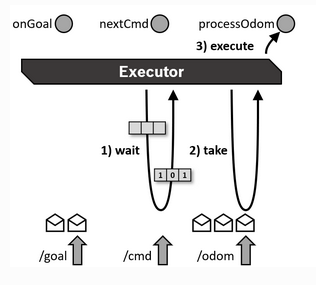
\includegraphics[width=0.6\textwidth]{imgs/ROS2_executor.png}
        \caption{ROS2 Executor}
        \label{fig:ros2_executor}%
    \end{figure}

    Anschließend wird der Executor in den 'Spin'-Modus versetzt in dem er einfach die verschiedenen Callbacks nach Bedarf ausführt.
    Damit ist die Initialisierung des Roboters abgeschlossen und er ist nun einsatzbereit.\\

    Wenn eine Nachricht empfangen wird, wird sie in einer globalen Variablen gespeichert.
    Auf diese Variable greift die Callback des Timers zu und führt wenn nötig die entsprechenden Änderungen durch.\\

    Zuerst werden die empfangenen Werte auf einen Bereich von -1 und +1 beschränkt um eine spätere Abbildung auf Registerwerte möglich zu machen.

    Danach werden die linearen und angularen Teile der Nachricht in Werte für die PWM-Channels umgewandelt.
    Dafür wird ein vorzeichenbehafteter Pythagoras aus den Werten der linearen und angularen Richtung berechnet.
    Durch abziehen bzw. addieren der linearen und angularen Teile je nach Radseite wird so die Message in Werte umgewandelt, mit denen der Roboter gesteuert werden kann.
    Ein Code-Beispiel für diese Berechnungen befindet sich in \ref{robot_code_snippet}.\newline

    Anschließend wird die Geschwindigkeit für die einzelnen Räder von den Eingabewerten zwischen -1 und 1 auf den Wertebereich der PWM-Channels abgebildet.
    Dabei gibt es einen Maximal und einen Minimalwert, mit dem man indirekt die Spannungen bestimmen kann, die man an den Motor anlegt.
    Der Maximalwert ist dabei nicht von so großer Bedeutung wie der Minimalwert, da die maximale Spannung, sowieso durch die Hardware bereits limitiert ist.
    Der Minimalwert muss allerdings durch Experimente herausgefunden werden, denn wenn man eine zu geringe Spannung an den Motor anlegt, die ihn nicht in Bewegung versetzt, kann das den Motor beschädigen.

    Zum Schluss werden die entsprechenden Registerwerte für die PWM-Signale noch gesetzt.

\end{flushleft}